%%==================================================
%% chapter01.tex for BIT Master Thesis
%% modified by 朱杰
%%==================================================
\chapter{相关工作}
\section{社交网络}
\subsection{社交网络的定义}
在维基百科中,社交网络(Social network)被定义为“由许多节点以及节点间关系构成的一个网络结构。节点通常是指个人或组织(又称社团),社交网络代表各种社会关系”。直白简洁的说,社交网络其实就是在互联网上与其他人相联系的一个平台。对社交网络的分析在早期只是针对现实生活中切实的方便调查的关系进行分析。比方说:早期在国外曾有研究人员在研究如何减少政府机构的冗余行政人员以提高办事效率和降低政府开销时,就使用到了社交网络分析这一手段。他们采用私下采访和调查的手段获取了某一政府机关几乎全部工作人员之间的来往接触关系,建立了一张交际网络。通过对这张交际网络的分析发现,其中有些节点在业务流程线上是属于多余的,其功能只是交接两边的节点。对于提高效率而言,分析此网络并减少这样无谓的节点即可有效的降低开销。不像早期的社交网络主要是通过合作关系建立起来的职业网络,如今随着互联网社交媒体的诞生和飞速发展,社交网络逐渐线上化。

本文所指的社交网络特指在线社交网络(下文统称社交网络)。直白简洁的说,在线社交媒介其实就是在互联网上与其他人产生联系的一个平台。在线社交媒体主要有即时通讯类软件(比如微信、QQ)、在线社交类软件(比如Facebook、人人网)、微博类软件(比如新浪微博、Twitter)、贴吧类软件(比如百度贴吧、悟空问答、知乎)、博客分享类软件(比如CSDN、简书)、职场关系类软件(比如领英、脉脉)和短视频分享类(比如抖音、快手)等等。而社交网络就是在这些社交媒介中抽象虚拟出来的一张网络图,在这张图中,每个个人或者组织抽象为一个节点,而人与人之间的关系或者互动则抽象为边。每个账号在社交媒体上填写的个人信息就是其节点属性,同样节点彼此之间的边上也有着相应的边的属性。这一切就构成了一个社交网络结构。网络虽然都是抽象出来的,但是这些关系却又都是真实的。图\ref{fig:fig2-0}展示了一个简单的社交网络抽象图。

\begin{figure}
  \centering
  
\includegraphics[width=0.75\textwidth]{figures/fig2-0}
  \caption{一个简单的社交网络抽象图}\label{fig:fig2-0}
\end{figure}

在种类繁多各色各样的在线社交媒体中,人们的参与度也越来越高。2017年Q3微博财报数据显示,截至2017年9月,微博月活跃用户共3.76亿;2018年1月15日,在广州举行的微信公开课上微信创始人、腾讯高级副总裁张小龙指出微信用户量已超10亿;而国外的Facebook更是早在2017年就已超20亿用户。社交网络具有传播迅速、传播广泛、自发性和言论相对自由等特点。面对这么巨大的用户量,不仅仅是普通个人用户,我们可以发现在诸多知名在线平台上各类官方媒体也都已入驻,以借助传播更加快捷和广泛的在线社交媒介来进行宣传等目的。当然,因为用户量的越发增加,在线社交媒介的广泛使用带来的问题也越来越多。这也对社交网络的规范化和整治不断提出挑战。

在现在这样的背景下,已经越发明显的出现线上影响线下的这种趋势。在人们享受社交网络带来的乐趣和便利之时,同样也有不法分子为了金钱或其他利益利用社交网络缺乏规范又利于传播等特点进行违法犯罪,包括诈骗、散布暴力恐怖信息或谣言等等。最近国家广电总局也整治了一大批社交媒体,封杀了一系列严重违规的软件,即使是今日头条、抖音、快手这样的大公司也面临着很大的危机,被勒令整改。因此,为了更好的利用社交网络给人们带来的便捷,同时又能避免产生危害,就产生了社交网络分析(social network analysis)这一研究领域。它是一门横跨信息学、数学、计算机技术、社会学、管理学和心理学等学科的交叉科学,主要研究的是社交网络的网络结构和其演化、社交网络中的群体及其互动、社交网络中的信息及其传播。

\subsection{社交网络的统计特性}

社交网络模型许多概念来自于图论,因为社交网络模型本质上是一个由节点(人)和边(社交关系)组成的图。笔者将简要介绍社交网络模型中常用的统计概念。

度(Degree):节点的度定义为与该节点相连的边的数目。在有向图中,所有指向某节点的边的数量叫作该节点的入度,所有从该节点出发指向别的节点的边的数量叫作该节点的出度。网络平均度反应了网络的疏密程度,而通过度分布则可以刻画不同节点的重要性。

网络密度(Density):网络密度可以用于刻画节点间相互连边的密集程度,定义为网络中实际存在边数与可容纳边数上限的比值,常用来测量社交网络中社交关系的密集程度及演化趋势。

聚类系数(Clustering Coefficient):用于描述网络中与同一节点相连的节点间也互为相邻节点的程度。其用于刻画社交网络中一个人朋友们之间也互相是朋友的概率,反应了社交网络中的聚集性。

介数(Betweeness):为图中某节点承载整个图所有最短路径的数量,通常用来评价节点的重要程度,比如在连接不同社群之间的中介节点的介数相对于其他节点来说会非常大,也体现了其在社交网络信息传递中的重要程度。

\subsection{社交网络的典型特征}

小世界现象:小世界现象是指地理位置相距遥远的人可能具有较短的社会关系间隔。早在1967年,哈佛大学心理学教授 Stanley Milgram 通过一个信件投递实验,归纳并提出了“六度分割理论(Six Degrees of Separation)”,  即任意两个都可通过平均五个人熟人相关联起来。1998年,Duncan Watts 和 Steven Strogatz 在《自然》杂志上发表了里程碑式的文章《Collective Dynamics of “Small-World” Networks》,该文章正式提出了小世界网络的概念并建立了小世界模型。

小世界现象在在线社交网络中得到了很好地验证,根据2011年 Facebook 数据分析小组的报告, Facebook 约7.2亿用户中任意两个用户间的平均路径长度仅为4.74,而这一指标在推特中为4.67。可以说,在五步之内,任何两个网络上的个体都可以互相连接。

无标度特性:大多数真实的大规模社交网络都存在着大多数节点有少量边,少数节点有大量边的特点,其网络缺乏一个统一的衡量尺度而呈现出异质性,我们将这种节点度分布不存在有限衡量分布范围的性质称为无标度。无标度网络表现出来的度分布特征为幂律分布,这就是此类网络的无标度特性。

\section{社区发现}

社区发现(community detection,也可以译作社区检测)是一个复杂而有意义的过程,它对研究复杂网络的特性具有重要作用。给定一个网络图,找出其社区结构的过程就叫做社区发现。近几年,发现及分析复杂网络中的社区结构得到了许多学者的关注,同时也出现了很多的社区发现算法。

\subsection{社区结构定义}

(1)一般社区结构定义

目前对网络社区的定义还没有一个统一的标准,人们从不同的角度给出了不同的社区结构的定义。典型的包括:基于子图的局部定义和基于节点相似度的定义。

基于子图的局部定义:社区结构可以被看成网络拓扑结构中具有高内聚特点的若干节点集合,这些节点集合往往是某种具有独立功能或者性质的相对独立组件的抽象。因此,可以根据网络局部拓扑结构特点来定义社区结构。当前,被各领域学者广泛接受的一个描述定义是基于子图的局部定义。即社区结构是复杂网络节点集合的若干子集,每个子集之间的节点之间连接非常紧密,不同子集的节点之间连接比较稀疏,如图\ref{fig:fig2-1}所示。图中的网络由20个节点组成,这20个节点被划分成了三个社区结构,分别对应着图中的三个虚线内部的结构。

\begin{figure}
  \centering
  
\includegraphics[width=0.75\textwidth]{figures/fig2-1}
  \caption{一个具有社区结构的网络示意图}\label{fig:fig2-1}
\end{figure}

 基于节点相似度的定义:从物理意义上讲,社区往往代表了复杂系统或者复杂网络中的具有相似或者相同功能的元素集合,这些元素相互协作或者相互作用,共同完成整个系统中某些相对独立的功能或者组织结构。据此,可以基于节点的相似度来定义社区,该定义假定社区内部节点都是相似的,社区间的节点相似性低,采用某种指标来衡量网络节点间的相似性,根据节点之间的相似性来定义社区结构。总体而言,从本质内涵来看,已有的社区结构的定义都是一致的,是由网络中所有个体组成的集合的子集,该集合中的个体基于某种属性连接紧密并和子集外的个体连接稀疏。但是紧密和稀疏并没有一个可以定量分析的标准,这些定义就没有多少实用的价值。

 (2)重叠社区结构定义

	在真实世界的社交网络中,社区结构呈现复杂多样的特点,大部分社区结构是重叠的,这就是说网络的节点集合中存在一些同时属于多个社区的节点,即重叠节点。比如,在社交网络中一个个体可以同时属于多个社会团体,各个组织之间有一些共有的个体。在各种类型的网络中,重叠节点一般十分重要。所以,网络中的重叠社区发现获得了越来越多人的关注。
  
  通常,重叠社区结构大致被分为两种类型:离散重叠社区和模糊重叠社区。对于前者,我们只要判断一个节点属不属于一个社区,也就是说节点要么属于一个社区,要么不属于这个社区。相反,模糊重叠需要计算节点对于不同的社区的隶属度,对于某个社区的隶属度有高有低。

\subsection{社区网络模型描述}

网络中社区结构表示的是网络中节点集合的子集。一般情况下,一个复杂的网络可以这样表示:由顶点集 $V$和边集 $E$组成的图$G=(V,E)$。节点个数表示为$n=|V|$,边数表示为$m=|E|$。如果任意两个节点对 $(i, j)$ 与 $(j, i)$表示的是同一条边,该图被称为无向图,否则,该被称为有向图。如果我们给图中的每一条边都设置一个代表关系强弱程度的数值,我们把这种图定义为有权图;否则,该图被称为无权图。显然,我们也可以把无权图看成图中每条边权重值都相同的有权图,比如权值都为1。在无向图中的定义中,节点i的度指的是以i为顶点的边的数目,记为,是所有含有该节点的边的数量的总和。在有向图的定义中,节点的度分为两种类型,入度和出度。以该节点为终点的边的数量为该节点的出入度,以该节点为起点的边的数量为该节点的出度。在无向图中无出入度之分。此外,我们还可以用邻接矩阵或者邻接表来表示网络的真实拓扑结构,邻接矩阵如果是对称矩阵那么表示的是无向图,如果是非对称的矩阵表示就是有向图。

\section{社区结构评价指标}

迄今为止,出现了各种各样的社区发现算法,如何评价不同的的发现算法的好坏是一个非常重要的问题。为此,学者们提出了多种社区结构评价指标用来评价网络社区划分质量,其中比较有代表性的有模块度、NMI等。下面详细介绍这些指标。

\subsection{模块度}

模块度是目前学者们最常用和经典的网络社区结构评价指标,它最初是被Newman等人于2004年提出来的\cite{2002Community}。其通过比较现有网络和基准网络在相同社区划分下的连接密度差来衡量网络社区的优劣,其中基准网络是由原网络具有相同度序列的随机网络。模块度计算公式如下:

\begin{equation}
  \label{eqn:LBmodel}
  Q=\frac{1}{2m}\sum_{i,j}\left [ A_{ij}-\frac{k_ik_j}{2m} \right ]\delta (c_i, c_j)  
\end{equation}

其中,A 表示网络中的邻接矩阵, m 表示网络中边的总数,$k_i$和$k_j$表示节点 i 和 j 的度数,$c_i$和$c_j$表示节点 i 和 j 所属的社区。如果$i=j,\delta(c_i,c_j)=1$,反之$\delta(c_i,c_j)=0$

......

\subsection{NMI}

随着在线社交网络的发展,人们发现在线社交网络的很多数据中存在着暗示各个节点的社区属性信息。例如,在人人网的学校信息便揭示了网络节点中属于同一学校的社区结构,Facebook中的兴趣信息同样表征了具有相同兴趣的虚拟用户群体。这些数据在为社区发现问题提供了丰富的信息的同时,也在一定程度上为虚拟社区结构优劣的评判提供了标准答案。针对这种预先拥有一定虚拟社区结构信息的情况下,Leon Danon等人【34】提出了Normalized Mutual Information(NMI)利用信息化熵来衡量算法划分的社区结构和预先已知的社区结构之间的差异。NMI是基于混合矩阵(Confusion Matrix)N来计算的数字指标。NMI公式如下:

\begin{equation}
  \label{eqn:LBmodel}
  NMI=\frac{ -2 \sum_{i,j} N_{ij}  ln{\frac{N_{ij}}{N_iN_j}} } {\sum_{i}N_iln{\frac{N_i}{n}}+\sum_{j}N_jln{\frac{N_j}{n}}}
\end{equation}

使用该数字指标,可以衡量划分出来的社区结构与已知的网络社区结构的差异程度值,该值越大,则表明获得的社区结构划分越好,当该值达到最大化值1时,说明算法发现的社区结构与已知社区结构完全已知,效果最好。

\begin{figure}
  \centering
  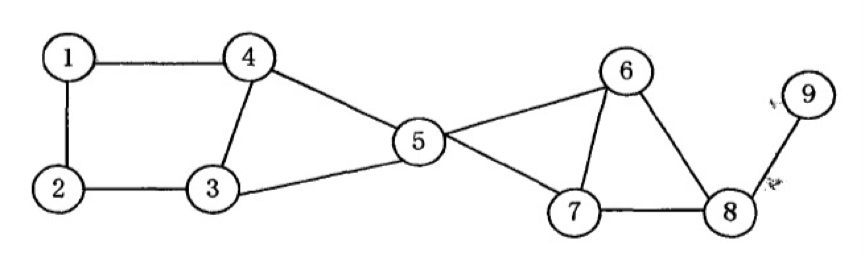
\includegraphics[width=0.75\textwidth]{figures/fig2-2}
  \caption{网络示例}\label{fig:fig2-2}
\end{figure}

下面以图\ref{fig:fig2-2}为例来说明计算NMI的过程。假设已知的最佳社区结构划分为集合{1,2,3,4}和{5,6,7,8},相应的社区划分向量表示为a = (1,1,1,1,2,3,3,3,3),再假设某算法获得的社区划分结构可以用向量表示为b = (3,3,3,3,2,1,1,1,1)来表示。根据已知的社区划分向量,可以构造混合矩阵N:

\begin{equation}
  \label{eqn:LBmodel}
  N=\begin{bmatrix}
    0 & 0 &4 \\ 
    0 & 1 & 0\\ 
    4 & 0 & 0
    \end{bmatrix}
\end{equation}

根据上式计算可知,该划分的NMI值为1。
